\documentclass{beamer}
\usepackage[utf8]{inputenc}
\usepackage[]{hyperref}
\usepackage{booktabs}
\usetheme[pageofpages=of,bullet=square,
	titleline=true,
	alternativetitlepage=true,
	titlepagelogo=images/xkcd-boyfriend2.jpg]{Torino}

\author{Statistical Reasoning\\and Quantitative Methods}
\title{Comparisons}
\institute{François Briatte \& Ivaylo Petev}
\date{Session 7}

\include{settings}

\begin{document}
		
	\begin{frame}[t,plain]
		\titlepage
	\end{frame}
	
	\begin{frame}[t]{Outline}
		
		\begin{columns}[T]
		\column{.35\textwidth}
			\tableofcontents[hideallsubsections]
		\column{.55\textwidth}
		\end{columns}

		\vspace{1em}
		
		\begin{center}
		\href{http://languagelog.ldc.upenn.edu/nll/?p=1107}{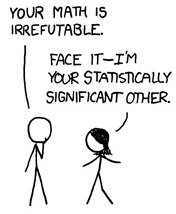
\includegraphics[scale=.35]{images/xkcd-boyfriend.jpg}}	
		\end{center}
					
	\end{frame}

	\section{Significance testing}

	\subsection{Hypothesis testing}

	\begin{frame}[t]{Hypothesis testing}
		
		\href{http://reason.org/}{From the Reason Foundation}, a ``free minds and free markets'' U.S. think tank:
			
		\begin{quote}
		``A number of theorists assume that drinking has harmful economic effects, but data show that \textbf{drinking and earnings are positively correlated}. \textbf{\red{We hypothesize that drinking leads to higher earnings by increasing social capital.}} If drinkers have larger social networks, their earnings should increase. Examining the General Social Survey, we find that self-reported drinkers earn 10-14 percent more than abstainers, which replicates results from other data sets.''\\
		(\href{http://reason.org/news/show/127594.html}{Bethany L. Peters and Edward Stringham, ``No Booze? You May Lose'', 2006.})
		\end{quote}

		\red{$H_1$:} ``An increase in social drinking causes an increase in earnings.''
	\end{frame}

	\fullslide{images/mad-men.jpg}

	\fullslide{images/booze.jpg}

	% Source: http://thinkprogress.org/yglesias/2011/08/11/293295/more-educated-people-spend-more-on-booze/ (Matthew Yglesias, data from the U.S. Bureau of Labour Statistics)
	
	\begin{frame}[t]{Hypothesis testing}

		\begin{itemize}
		\item Devise at least two reasons why the causality might run from high income to frequent social drinking, \red{rather than vice versa}. (Question by \href{http://www.cscs.umich.edu/~crshalizi/}{Cosma Shalizi}).
		\item Imagine a \red{non-linear relationship} between alcohol intake, income and employment opportunities in countries where social drinking is legal and generally accepted.
		\end{itemize}
		
		Formally, you first need to \textbf{reject the null hypothesis}:
		
		\red{$H_0$:} There is \red{no relationship} between social drinking and earnings.

		\red{$H_a$:} There is a relationship between social drinking and earnings.\vspace{1em}
		
		Your alternative hypothesis should be a \textbf{directional hypothesis}:\\
		$H_{a1}: \red{+} \textsf{social drinking}~(\rightarrow \textsf{+social capital}) \rightarrow \red{+} \textsf{earnings}$\\
		$H_{a2}: \red{+} \textsf{earnings}~(\rightarrow \textsf{+disposable income}) \rightarrow \red{+} \textsf{social drinking}$\\
		...
	\end{frame}	
	
	\subsection{Significance testing}
	
	\begin{frame}[t]{Significance testing}

	\begin{itemize}
		\item \textbf{Significance testing} starts with the \red{null hypothesis}:
		
			\begin{itemize}
				\item \red{$H_0$} asserts the absence of a relationship.
				\item \red{$H_a$} asserts the presence of a relationship.
			\end{itemize}

			Formally, $\Pr(H_0)+\Pr(H_a)=1$.

		\item \textbf{Proof by contradiction} works by \red{rejecting} the null hypothesis:
		
			\begin{itemize}
				\item $\alpha$ is a conventional \red{level of statistical significance}.
				\item $H_0$ is rejected when its \red{estimated probability} is lower than $\alpha$.
			\end{itemize}
			
			Conventionally, $\alpha = 0.05$.
				
		\item \textbf{Serious issues} occur when attaching $p$-values to hypotheses:
		
			\begin{itemize}
				\item Due to \href{http://en.wikipedia.org/wiki/Jeffreys-Lindley_paradox}{formal assumptions}, $p=.01 \nRightarrow \Pr(H_a)=.99$.
				\item Due to conventions, $H_0$ is rejected at $p = .051$, retained at $p = .049$.
			\end{itemize}
		
		$H_0$ can hence be \red{erroneously rejected or retained}.
		
	\end{itemize}

	\end{frame}
		
	\begin{frame}[t]{Significance testing}
			
		\begin{itemize}

			\item \textbf{Assumptions} behind significance tests:
			
				\begin{itemize}
					\item The \red{population distribution} is assumed to be \textit{approximately} normal: $X\ \sim\ \mathcal{N}(\mu,\,\sigma^2)$ by virtue of the Central Limit Theorem.	
					\item The \red{sample distribution} \textit{will} depart from the normal distribution to some extent, by virtue of the Law of Large Numbers.
					\item The \red{probability distribution}, like Student's $t$-distribution, reflects only an \textit{estimated} $p$-value for $H_0$.
				\end{itemize}
			
			\item \textbf{Errors} with significance tests:
			
				\begin{itemize}
					\item \textbf{Type I Error} rejects $H_0$ when it is actually \red{true}.
					\item \textbf{Type II Error} retains $H_0$ when it is actually \red{false}.
				\end{itemize}
		\end{itemize}

		You \textit{cannot} rule out the possibility that your significance test violates its background assumptions, and that you are hence making a Type I or Type II error when interpreting its results, even when $p \ll \alpha$.
	\end{frame}	

	\subsection{Type I and II Errors}
	
	\begin{frame}[t]{Type I and II Errors}
			
		\begin{itemize}

			\item \textbf{Type I Error} in judicial trials:\vspace{.5em}
			
			``Last year executed man proven innocent by DNA evidence.''
			
				\begin{itemize}
					\item $H_0$: presumption of innocence
					\item $H_a$: ... until proven guilty (\red{$H_0$ wrongly rejected})
				\end{itemize}
			
			\item \textbf{Type II Error} in child protection:\vspace{.5em}
			
			``Violent father beats children after being released from custody.''
			
				\begin{itemize}
					\item $H_0$: parents considered responsible
					\item $H_a$: ... until proven abusive (\red{$H_0$ wrongly retained})
				\end{itemize}
		\end{itemize}

		Proof by contradiction is \red{context-dependent}: a Type I Error can carry more serious consequences than a Type II Error, and vice versa.\vspace{1em}
		Medical trials provide some evidence of the risks of both Type I Errors (``tea $\rightarrow$ cancer'') and Type II Errors (``therapy $\rightarrow$ death'').
	\end{frame}	

	\section{Comparisons}

	\subsection{Comparing means}

	\begin{frame}[t]{Comparison of means \red{in the sample}}
					
		\begin{quote}
		``Girls suck at math.''
		\end{quote}
		
		Dependent variable: \red{continuous} standardised math score (\code{0-100})

		Independent variable: \red{binary} gender groups (\code{1 "Female" 0 "Male"})

		\begin{itemize}
			\item \textbf{Measurement} in two independent groups:

				\begin{itemize}
					\item \red{Mean} math score for men: $\bar{x}_{men}$ and women: $\bar{x}_{women}$
					\item \red{Difference} in mean scores: $\Delta_{scores} = \bar{x}_{men} - \bar{x}_{women}$
				\end{itemize}

			\item \textbf{Association} between gender and educational attainment:
									
				\begin{itemize}
					\item $H_0: \red{\Delta_{scores} = 0} \Leftrightarrow \bar{x}_{men} - \bar{x}_{women} = 0$ (no significant difference)
					\item $H_a: \red{\Delta_{scores} \neq 0} \Leftrightarrow \bar{x}_{men} - \bar{x}_{women} \neq 0$ (significant difference)
%					\item \red{Reject} $H_0$ if $Pr(H_0: \Delta_{scores}=0) < \alpha$, i.e. $Pr(\textsf{Type I Error})<1-\alpha$
%					\item \red{Retain} $H_0$ if $Pr(H_0: \Delta_{scores}=0) > \alpha$, i.e. $Pr(\textsf{Type II Error})<1-\alpha$
				\end{itemize}
			
			\item \textbf{Direction} of the alternative hypothesis: 
						
				\begin{itemize}
					\item $H_{a1}: \red{\Delta_{scores} > 0} \Leftrightarrow  \bar{x}_{men} > \bar{x}_{women}$ (men outperform women)
					\item $H_{a2}: \red{\Delta_{scores} < 0} \Leftrightarrow  \bar{x}_{men} < \bar{x}_{women}$ (women outperform men)
				\end{itemize}
		\end{itemize}

	\end{frame}	

	\begin{frame}[t]{Comparison of means by \red{estimation}}
					
		\begin{quote}
		``Girls suck at math.'' $\Leftrightarrow Pr(\Delta_{scores} \neq 0) = \red{1 - Pr(H_0)}$
		\end{quote}
		
		A \textbf{``\textit{p}-value''} designates the \red{probability level of the null hypothesis}.\\[1em]
		
		\red{A significance test rejects $H_0$} when $Pr(H_0) < \alpha \Leftrightarrow p < \alpha \Leftrightarrow \red{p < .05}$ when $\alpha$, your \textbf{level of statistical significance}, is at 95\% \textbf{confidence} (the conventional standard for our course of study):
		
		\begin{itemize}
			\item \textbf{Reject $H_0$} if $Pr(\Delta_{scores}=0) < 0.05 \Leftrightarrow \red{Pr(H_0) < \alpha}$.
			
			\begin{itemize}
				\item $H_0$ is wrongly rejected in \textit{at most} $\alpha = 5\%$ of the cases (Type I Error).
				\item $H_a$ is estimated \red{significant} \textit{at least} at $1-\alpha=95\%$ confidence.
			\end{itemize}

			\item \textbf{Retain $H_0$} if $Pr(\Delta_{scores}=0) > 0.05 \Leftrightarrow \red{Pr(H_0) > \alpha}$.\\
			\begin{itemize}
				\item $H_0$ is wrongly retained in $\alpha = 5\%$ of the cases (Type II Error).
				\item $H_a$ is estimated \red{insigificant} \textit{at least} at $1-\alpha=95\%$ confidence.
			\end{itemize}
		\end{itemize}
	\end{frame}	

	\begin{frame}[t]{Comparison of means by \red{statistical significance}}
					
		\begin{quote}
		``Girls suck at math.''\\
		$\Leftrightarrow$ \textbf{rejected} if $\red{p > .05} \Leftrightarrow Pr(H_0) > \alpha$ (significance)\\
		$\Leftrightarrow$ \textbf{accepted} if $p < .05 \Leftrightarrow Pr(H_0) < \red{1-\alpha}$ (confidence)
		\end{quote}

		\begin{itemize}
 			\item A significance test \textbf{can only reject the null hypothesis} by \red{estimating} its $p$-value, which \textit{you} then choose to reject or retain \textit{via} the level of confidence at which you estimate your hypotheses.
 			\item A significance test \textbf{cannot prove the alternative hypothesis}, because that interpretation is \textit{your} initiative after reading the \red{estimated} probability of the null hypothesis.
 			\item A significance test \textbf{cannot attach a p-value to a hypothesis}, since probability levels are \red{estimations} based on the null hypothesis.\\
 			The \textit{``$p < .05~\textsf{good, rest bad}$''} cargo cult is irresponsible.	
		\end{itemize}
	\end{frame}
	
	\subsection*{The Prophecy}

% img-longcat-tao.jpg

	% The efforts to raise the powers of Estimation Cat are considerable...
	\fullslide{images/longcat-prophecy1.jpg}

	\begin{frame}[t]{The Prophecy}

	The Prophecy requires \textbf{raising the power of \red{Estimation Cat}}\\as much as possible:
	
	\begin{columns}[T]
		\column{.625\textwidth}
		\begin{itemize}
 			\item \textbf{Maximise sample size:} missing observations and/or low $n$ reduce the \red{statistical power} of your sample.

 			\item \textbf{Approach normality:} Estimation Cat is pleased when your variables follow a \red{normal distribution}.

 			\item \textbf{Use the appropriate test:} significance tests come with \red{restrictive assumptions}, e.g. independent groups, equal variance.
		\end{itemize}

	This is difficult: Estimation Cat is needy.	

		\column{.3\textwidth}
	\vspace{0em}
	\begin{flushright}
	\includegraphics[scale=.3]{images/longcat.jpg}		
	\end{flushright}
	\end{columns}
		
	\end{frame}

	% ... But the threat of Significance Cat looms over the mere mortal researcher.
	\fullslide{images/longcat-prophecy2.jpg}

	\begin{frame}[t]{The Prophecy}

	The Prophecy also requires \textbf{curbing the threat of \red{Significance Cat}} as much as possible:
	
	\begin{columns}[T]
		\column{.625\textwidth}
		\begin{itemize}
 			\item \textbf{Maximise sample size} (again): the number of observations restricts the \red{degrees of freedom} used to calculate $p$-values from \red{Student's $t$-distribution}.

 			\item \textbf{Use the appropriate test} (again): a correct reading of an inappropriate test is a \red{Type III Error} (providing the right answer to the wrong question).
		\end{itemize}

	This is also difficult, especially given the cunning nature of Significance Cat.	

		\column{.3\textwidth}
	\vspace{0em}
	\begin{flushright}
	
\includegraphics[scale=.3]{images/longcat-black.jpg}		
	\end{flushright}
		
	\end{columns}
	\end{frame}
	
	\begin{frame}[t]{The Prophecy}

	The Prophecy is chiefly achieved through \textbf{statistical reasoning} that carefully balances the awesome powers of \red{estimation} and \red{significance}:
	
	\begin{columns}[T]
		\column{.625\textwidth}
		\begin{itemize}
 			\item \textbf{Keep an open mind}: reading $p$-values require paying attention to \red{Type I and Type II Errors}. The key to any test remains interpretation.

 			\item \textbf{Avoid cargo cults:} statistical inference is a probabilistic method. Each test result is expressed as a \red{likelihood} that carries no absolute certainty.
		\end{itemize}
		\column{.3\textwidth}
	\vspace{0em}
	\begin{flushright}
	
\includegraphics[width=\textwidth]{images/longcat-tao.jpg}		
	\end{flushright}		
	\end{columns}
	
		\vspace{1em}
		And yes, this amounts to a lot of computational and intellectual effort for the incomplete and imperfect results of frequentist statistics.	
		
	\end{frame}

	\subsubsection{ttest}

	\begin{frame}[t]{Stata implementation: \textit{t}-test (means)}

	Compare the average literacy rates of democracies and dictatorships.\\[1em]
	
	% From 3.5% to 7% female leaders if you manipulate the regime type: the proportion doubled. 
	\includegraphics[width=\textwidth]{images/comp-means1.pdf}
	\end{frame}

	\begin{frame}[t]{Stata implementation: \code{ttest}}
	
	\includegraphics[width=\textwidth]{images/comp-means2.pdf}\\[1em]
	
	Read the \red{confidence interval of the difference}: the interval does not include 0, indicating a statistically significant difference.
	\end{frame}
	
	\subsection{Comparing proportions}

	\begin{frame}[t]{Comparison with \red{proportions}}
					
		\begin{quote}
		``Scotland has the most redheads.''
		\end{quote}
		
		Dependent variable: \red{binary} hair colour (\code{1 "Red" 0 "Other"})

		Independent variable: \red{binary} location (\code{1 "Scotland" 0 "Other"})

		\begin{itemize}
			\item \textbf{The mean of the dependent variable \textit{reads} as a proportion:} e.g. a mean of $\bar x=.13$ indicates a proportion of 13\% of redheads.

			\item \textbf{Yet proportions are not \textit{statistically assimilable} to means:} having red hair is not a continuous but a binary yes/no attribute.
			
			\item \textbf{A different distribution therefore applies to binary variables:} the binomial distribution is used instead of the normal distribution. The rest of the mechanics are identical:
						
				\begin{itemize}
					\item The \red{proportion} $p$ of $N$ observations provides a standard error.
					\item The \red{difference in proportions} $\Delta_{p-q}$ provides a confidence interval.
					%  $\sqrt{\frac{p+q-(p-q)^2}{n}}$
					\item The \red{margin of error} is half the width of the confidence interval.
				\end{itemize}
		\end{itemize}

	\end{frame}	
	
	\subsubsection{prtest}

	\begin{frame}[t]{Stata implementation: proportions}

	Do parliamentary regimes select more female leaders?\\[1em]
	
	% The 95% CI includes 0.
	\includegraphics[width=\textwidth]{images/comp-prop1.pdf}\\[1em]
	
	Use \code{tab} (\code{tabulate}) to draw a $2 \times 2$ \red{contingency table}, with added column percentages (\code{col}) to read proportions of female leaders.
	\end{frame}

	\begin{frame}[t]{Stata implementation: \code{prtest}}
	
	\includegraphics[width=\textwidth]{images/comp-prop2.pdf}\\[0em]
	
	The difference in proportions is \red{statistically insignificant} at $p < .05$, even though it might be \red{substantively significant} (Type II Error).
	\end{frame}

\end{document}

